\section{Introduction}

In this chapter, we will focus on \gls{active} devices registered in Carbon Black Cloud.\\

\begin{tipblock}
How to ensure a Clean Inventory in Carbon Black Cloud? See 
\href{https://carbonblack.vmware.com/blog/automate-cleanup-deregistered-endpoints}{Automate the Cleanup of Deregistered Endpoints}
\end{tipblock}

\section{Active devices OS}

Only \gls{active} devices:

\nicecounter{123}{WINDOWS}
\nicecounter{8}{MAC}
\nicecounter{35}{LINUX}
\nicecounter{14}{Kubernetes clusters}


 \begin{noteblock}
Info: Some Linux devices may be Kubernetes nodes, \gls{cndr} automatically protect Kubernetes nodes.
\end{noteblock} 

For a complete list of supported operating systems, see \href{https://docs.vmware.com/en/VMware-Carbon-Black-Cloud/services/cbc-endpoint-standard-oer/GUID-45BFDC75-748B-4E05-8B38-190B59204D0B.html}{VMware Docs}.\\

%\newpage

%\section{Active devices OS versions}

%Only \gls{active} devices:

%\begin{figure}[H]
\begin{tikzpicture}
\begin{axis}[
xbar,
y axis line style = { opacity = 0 },
axis x line       = none,
tickwidth         = 0pt,
ytick             = data,
width=0.7\textwidth,
height=100pt,
symbolic y coords = {Windows 11 x64,Ubuntu 22.04.3 x64,Linux (Unsupported),},
nodes near coords
]
\addplot coordinates { (1,Windows 11 x64) (1,Ubuntu 22.04.3 x64) (1,Linux (Unsupported)) };
\end{axis}
\end{tikzpicture}
\caption{OS versions for active devices}
\end{figure}



%\section{Active devices sensor versions}

%Read this \href{https://carbonblack.vmware.com/resource/secure-carbon-black-cloud-updates}{article} to understand how to secure Carbon Black updates.\\
%\\
%Only \gls{active} devices:

%\subsection{Linux sensors}
\begin{figure}[H]
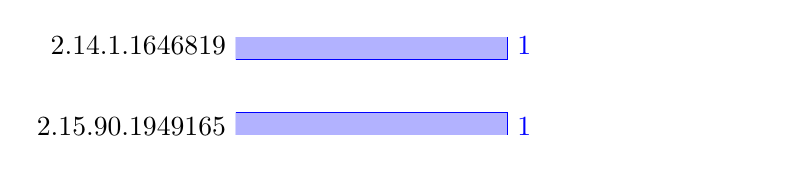
\begin{tikzpicture}
\begin{axis}[
xbar,
y axis line style = { opacity = 0 },
axis x line       = none,
tickwidth         = 0pt,
ytick             = data,
width=0.7\textwidth,
height=80pt,
symbolic y coords = {2.15.90.1949165,2.14.1.1646819,},
nodes near coords
]
\addplot coordinates { (1,2.15.90.1949165) (1,2.14.1.1646819) };
\end{axis}
\end{tikzpicture}
\caption{Linux sensor versions for active devices}
\end{figure}

\subsection{Windows sensors}
\begin{figure}[H]
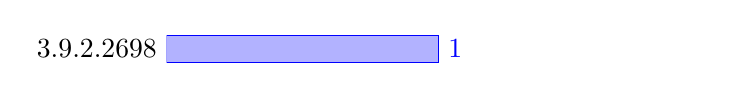
\begin{tikzpicture}
\begin{axis}[
xbar,
y axis line style = { opacity = 0 },
axis x line       = none,
tickwidth         = 0pt,
ytick             = data,
width=0.7\textwidth,
height=60pt,
symbolic y coords = {3.9.2.2698,},
nodes near coords
]
\addplot coordinates { (1,3.9.2.2698) };
\end{axis}
\end{tikzpicture}
\caption{Windows sensor versions for active devices}
\end{figure}



%\section{Active devices target values}

%Only \gls{active} devices are shown:

%\nicecounter{0}{LOW}
\nicecounter{1}{MEDIUM}
\nicecounter{2}{HIGH}
\nicecounter{0}{MISSION CRITICAL}


%\begin{tipblock}
%Hint: Your active directory server, database.. and all your critical assets should be in "MISSION CRITICAL" target value. The alert score will be increased based on the target value !
%\end{tipblock}


\section{Active devices quarantined}

Only \gls{active} devices are shown:

\nicecounter{0}{Quarantined devices}


\begin{tipblock}
 \href{https://community.carbonblack.com/t5/Knowledge-Base/Carbon-Black-Cloud-How-to-Quarantine-a-Device-from-the-Carbon/ta-p/71739}{How to quarantine a device?}
\end{tipblock}

\begin{tipblock}
	\href{https://community.carbonblack.com/t5/Knowledge-Base/Endpoint-Standard-What-happens-when-a-Device-is-placed-in/ta-p/71741}{What happens when a Device is placed in Quarantine?}
\end{tipblock}


\section{Active devices sensor out of date}

Only \gls{active} devices are shown:

\nicecounter{1}{Sensors out of date}


Read this \href{https://carbonblack.vmware.com/resource/secure-carbon-black-cloud-updates}{article} to understand how to secure Carbon Black updates.\\
